\paragraph{U-Net (2015)}\label{sec:u-net}

U-Net is a deep learning architecture introduced by Olaf Ronneberger et al. in 2015 for biomedical image segmentation tasks \cite{ronneberger_u-net_2015}. The name \textit{U-Net} comes from the shape of the network, which resembles the letter \textit{U}.

The U-Net architecture consists of two main parts: an encoder path and a decoder path. The encoder path is a typical \ac{CNN} (Section \ref{sec:CNN}) that extracts features from the input image. On the other hand, the decoder path uses upsampling operations to recover the spatial resolution of the feature maps and generate a segmentation mask. Upsampling is the process of increasing the resolution of an image or signal by using, for instance, nearest neighbor interpolation, bilinear interpolation, or transposed convolution (see Section \ref{sec:transpoed-conv}). The U-Net architecture can be seen in Figure \ref{fig:u-net}.

\begin{figure}[ht]
    \centering
    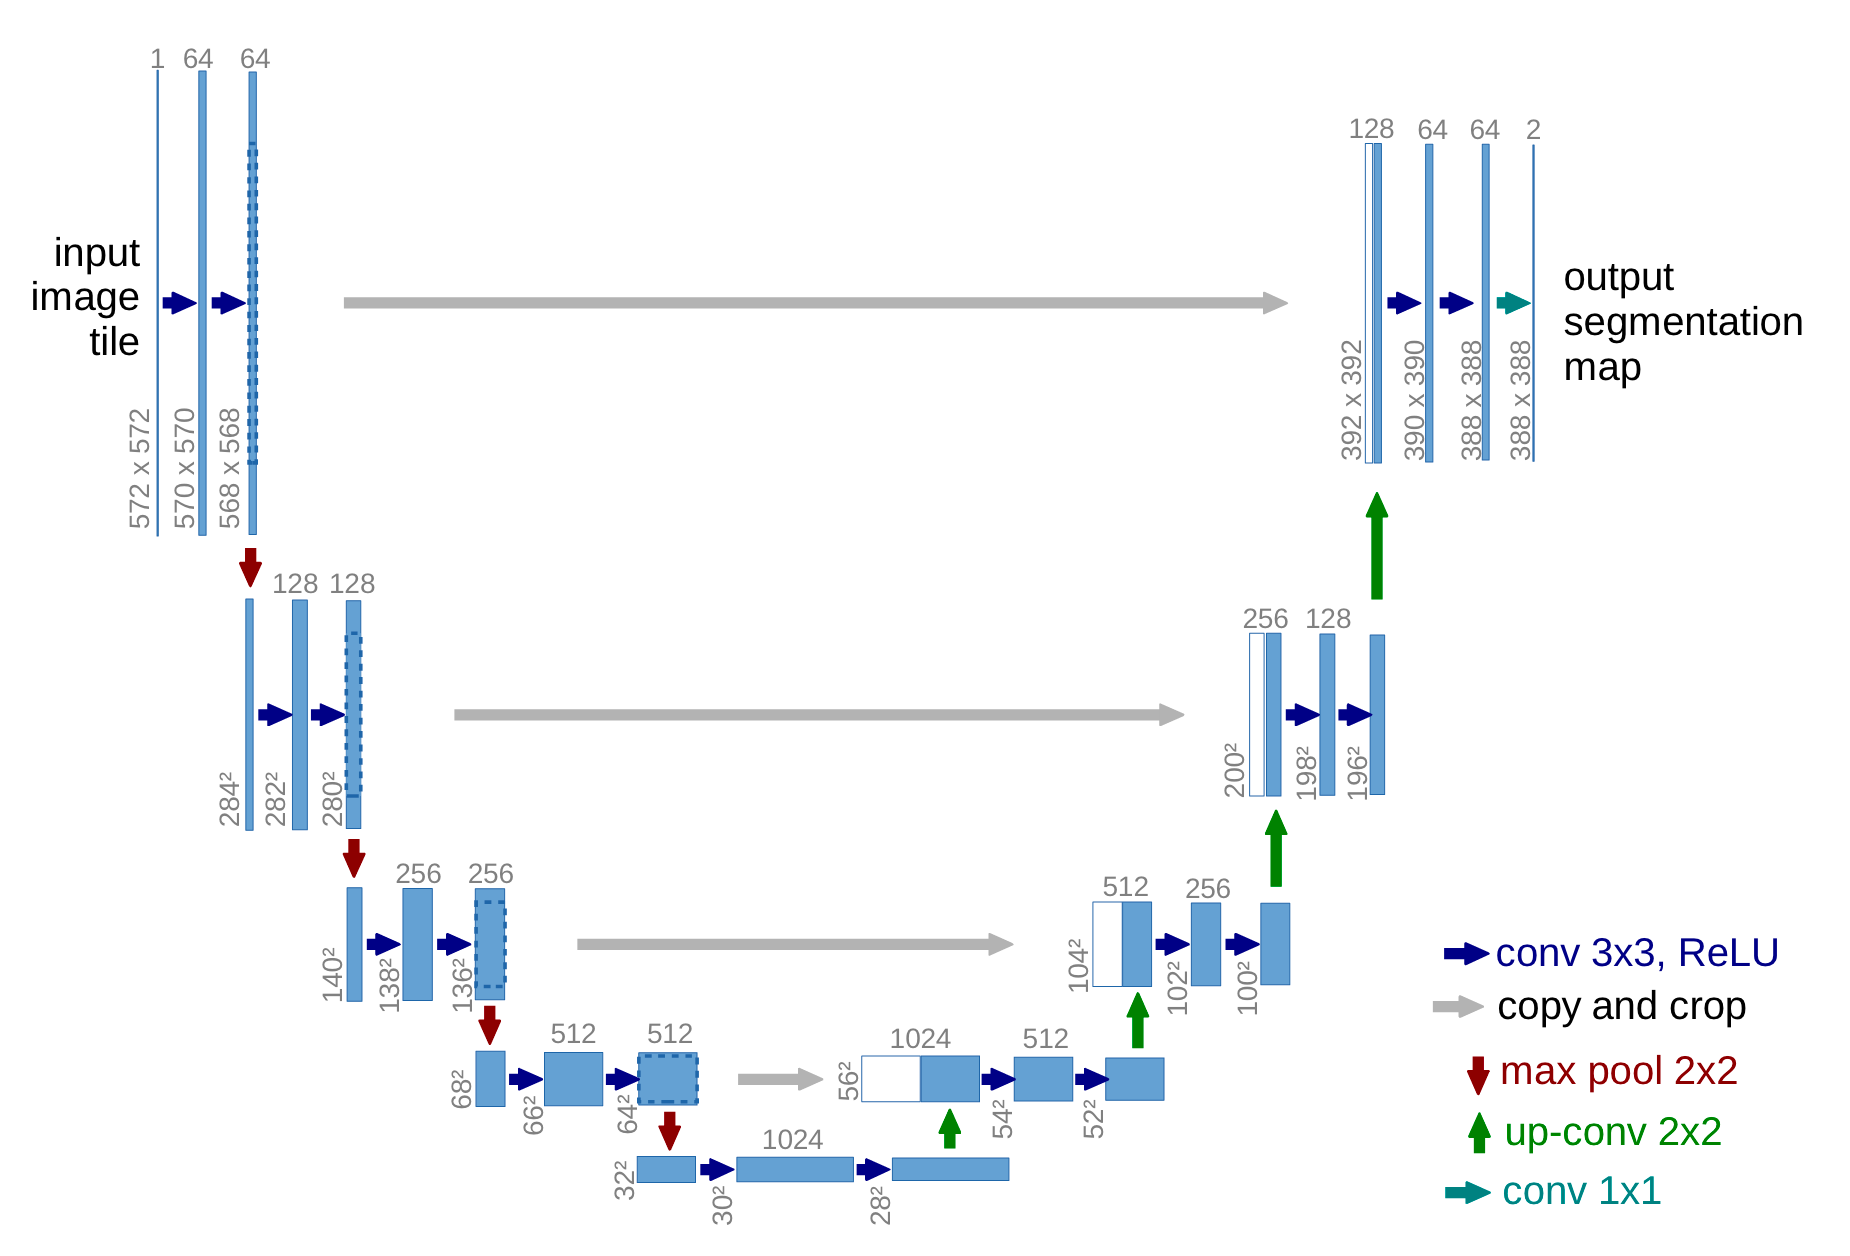
\includegraphics[width=\textwidth]{figures/2-sota/u-net/u-net.png}
    \caption[U-Net]{\textbf{U-Net} --- This figure was taken from the original paper and follows an example for images with $572 \times 572$ pixels. Each blue box corresponds to a multi-channel feature map. The number of channels is denoted on top of the box. The x-y-size is provided at the lower left edge of the box. White boxes represent copied feature maps. The arrows denote the different operations. One can see that at its smallest size, the feature maps were $28 \times 28 \times 1024$, and the end result provides two features maps of $388 \times 388$ pixels, meaning that this specific network could be used, for instance, for segmentation of foreground vs. background. It is also essential to notice that, to keep the original image's fidelity, there is a deconvolutional step for each convolutional one. These are concatenated (represented by the white boxes).}
    \label{fig:u-net}
\end{figure}

The encoder path extracts features from the input image. These features are then compressed into a lower-dimensional representation, which the decoder path uses to generate a segmentation mask for the input image. In this sense, the U-Net architecture can be viewed as a specialized type of \ac{AE} not designed to reconstruct the input image itself.

The U-Net architecture was initially designed to classify each pixel in an image as belonging to a specific object or background: image segmentation. It combines high-level and low-level features from the input image to generate the final segmentation.